\documentclass[]{article}
\usepackage[T1]{fontenc}
\usepackage[utf8]{inputenc}
%\usepackage[icelandic]{babel}
\usepackage{caption}
\usepackage{circuitikz}
\usepackage{grffile} 
\usepackage[margin=1in]{geometry}

% grffile er pakki sem leifir manni að nota "" til þess að forðast að nota
% nafnið á myndinni með.
\usepackage{graphicx}
% \graphicspath{{images/}} Sýnir undir möppu þar sem myndirnar eru

\usepackage{hyperref}
%fyrirlinka - \url{www.....}
\begin{document}


\title{Formleg mál og reiknanleiki}
\author{Pétur}
\maketitle

\section*{1.}

\subsection*{a)}
no

\subsection*{b)}
yes

\section*{2.}

\subsection*{a)}
No, B contains the empty sting and A dose not.
\subsection*{b)}
No, B contains the empty string and C dose not.
\subsection*{c)}
yes it is the same language.

\section*{3.}

\subsection*{a)}
grep -x ".\textbackslash\{3\textbackslash\}*"

\subsection*{b)}
grep  "[\.CSV|\%\textbackslash.\%\textbackslash.\%]" test.txt

\subsection*{c)}
grep -x "[\.CSV|\textsuperscript{$\wedge$}.* .*@.*\textbackslash..*]" test.txt 


\subsection*{c)}
grep ".*@.*\textbackslash..*"  test.txt

\section*{4.}

<<<<<<< Updated upstream
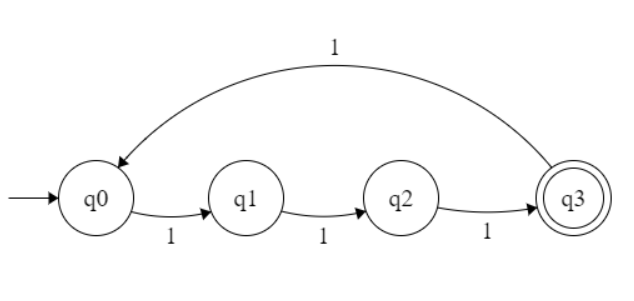
\includegraphics[scale=1]{mynd}

=======
\subsection*{a)}
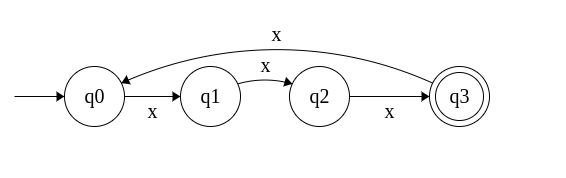
\includegraphics[scale=1]{myb}

\subsection*{b)}
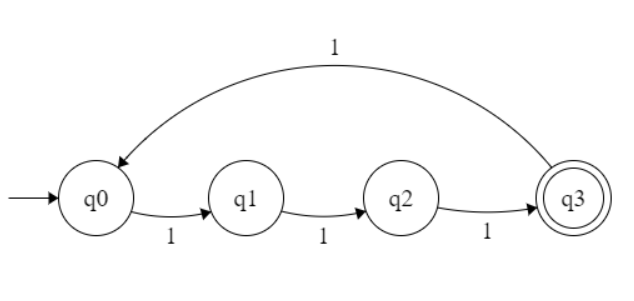
\includegraphics[scale=1]{mynd}

\subsection*{c)}

>>>>>>> Stashed changes


\end{document}